\documentclass[border=8pt]{standalone}
\usepackage{amsmath}
\usepackage{amssymb}
\usepackage{tikz}
\usetikzlibrary{arrows.meta,calc,decorations.pathreplacing,patterns,shapes.geometric,positioning,shadings,plotmarks}

\begin{document}
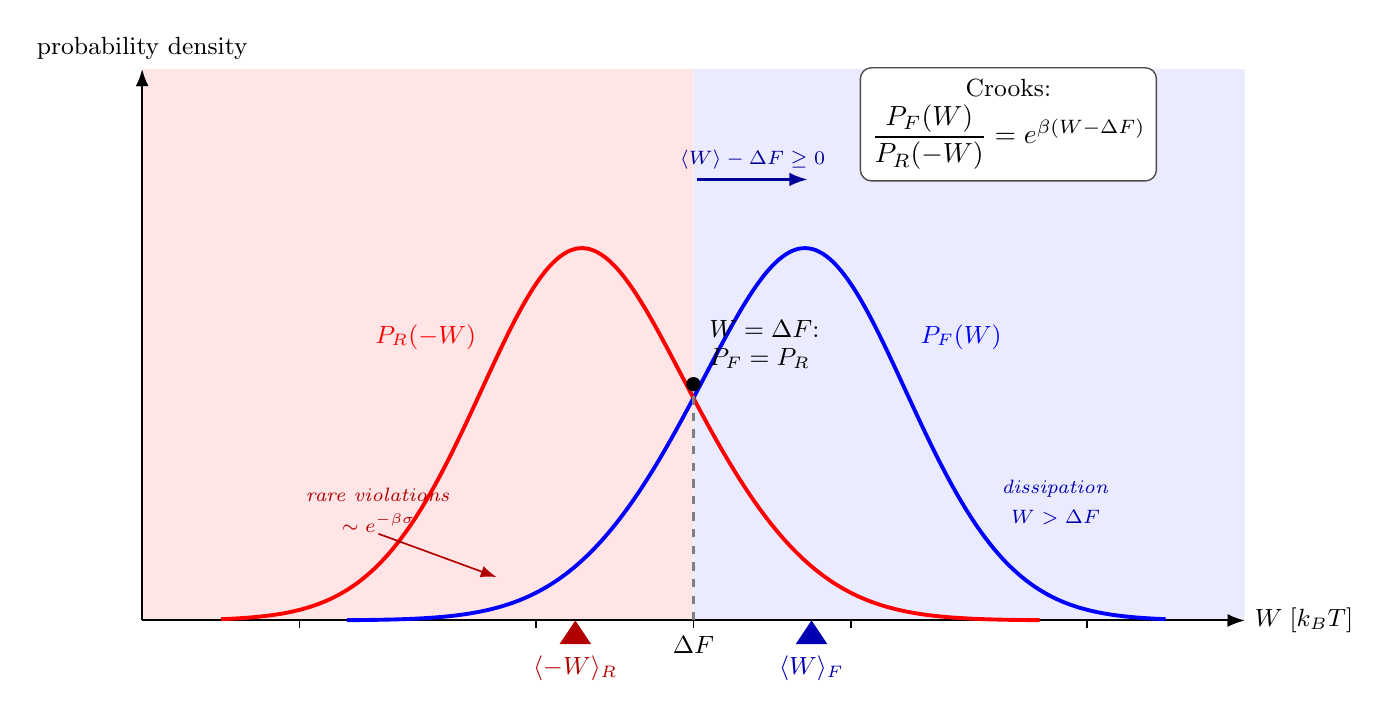
\begin{tikzpicture}[>=Latex,thick]

% --- Coordinate system ---
% Horizontal axis: W (in units of k_B T)
% Vertical axis: probability density
% Place crossing point at x = 7 (this is W = Delta F)
% Forward distribution P_F(W): mean ~ 8.5 (right of Delta F), right-skewed (tail to the right)
% Reverse distribution P_R(-W): mean ~ 5.5 (left of Delta F), left-skewed (tail to the left)
% Both must equal at x = 7 (Crooks: e^0 = 1, so heights match exactly)

% Axes
\draw[->, line width=0.7pt] (0,0) -- (14,0) node[right] {\small $W \;[k_B T]$};
\draw[->, line width=0.7pt] (0,0) -- (0,7) node[above] {\small probability density};

% Tick marks on horizontal axis
\foreach \x/\lab in {2/{}, 5/{}, 7/{}, 9/{}, 12/{}} {
  \draw[black, line width=0.5pt] (\x,0) -- (\x,-0.10);
}

% --- Shaded regions (background) ---
% Left region (W < Delta F): rare "second-law violating" events
\begin{scope}
  \clip (0,0) rectangle (7,7);
  \fill[red!10] (0,0) rectangle (7,7);
\end{scope}
% Right region (W > Delta F): dissipation
\begin{scope}
  \clip (7,0) rectangle (14,7);
  \fill[blue!8] (7,0) rectangle (14,7);
\end{scope}

% Re-draw axes on top
\draw[->, line width=0.7pt] (0,0) -- (14,0);
\draw[->, line width=0.7pt] (0,0) -- (0,7);

% --- Forward distribution P_F(W): right-skewed Gaussian-like, peaked near 8.0 ---
% Construct so curve passes through (7, 3.0) (the crossing height)
% Peak at ~8.0 with height ~4.5, with mild right skew (longer right tail)
% Use a piecewise-like construction: smooth bell with extra right-tail decay
\draw[blue, line width=1.4pt, smooth, samples=240, domain=2.6:13.0]
  plot (\x, { 4.5 * exp( -((\x-8.0)*(\x-8.0)) / (2.0*1.45*1.45) ) * (1 + 0.35*tanh( (\x-8.0)/1.5 )) });

% --- Reverse distribution P_R(-W): left-skewed Gaussian-like, peaked near 6.0 ---
% Mirror-skewed: longer left tail; passes through (7, 3.0)
\draw[red, line width=1.4pt, smooth, samples=240, domain=1.0:11.4]
  plot (\x, { 4.5 * exp( -((\x-6.0)*(\x-6.0)) / (2.0*1.45*1.45) ) * (1 - 0.35*tanh( (\x-6.0)/1.5 )) });

% --- Crossing point at W = Delta F ---
% Vertical dashed line down to axis
\draw[gray, dashed, line width=0.8pt] (7, 0) -- (7, 3.0);
% Crossing dot
\fill[black] (7, 3.0) circle (2.6pt);

% Label W = Delta F on axis
\node[below=2pt] at (7, 0) {\small $\Delta F$};

% Label crossing point
\node[above right=2pt and 2pt, align=left] at (7, 3.0)
  {\small $W = \Delta F$:\\[-2pt]\small $P_F = P_R$};

% --- Curve labels ---
\node[blue] at (10.4, 3.6) {\small $P_F(W)$};
\node[red]  at (3.6, 3.6) {\small $P_R(-W)$};

% Mean markers (small triangles on axis)
% Forward mean ~ 8.5
\fill[blue!70!black] (8.5, 0) -- (8.7, -0.30) -- (8.3, -0.30) -- cycle;
\node[blue!70!black, below] at (8.5, -0.32) {\small $\langle W\rangle_F$};
% Reverse mean ~ 5.5
\fill[red!70!black] (5.5, 0) -- (5.7, -0.30) -- (5.3, -0.30) -- cycle;
\node[red!70!black, below] at (5.5, -0.32) {\small $\langle -W\rangle_R$};

% --- Arrow showing dissipation gap ---
\draw[->, >=Latex, line width=0.8pt, blue!60!black]
  (7.05, 5.6) -- (8.45, 5.6);
\node[blue!60!black, above] at (7.75, 5.6)
  {\scriptsize $\langle W\rangle - \Delta F \ge 0$};

% --- Annotation for "violation" tail (left, small area) ---
\node[red!70!black, align=center] at (3.0, 1.4)
  {\scriptsize \textit{rare violations}\\[-1pt]\scriptsize $\sim e^{-\beta\sigma}$};
\draw[->, >=Latex, line width=0.6pt, red!70!black]
  (3.0, 1.10) -- (4.5, 0.55);

% --- Annotation for dissipation region ---
\node[blue!70!black, align=center] at (11.6, 1.5)
  {\scriptsize \textit{dissipation}\\[-1pt]\scriptsize $W > \Delta F$};

% --- Inset box (top right): Crooks formula ---
\node[draw=black!70, rounded corners, line width=0.5pt, align=center,
      fill=white, inner sep=4pt]
  at (11.0, 6.3)
  {\small Crooks: \\[2pt]
   $\dfrac{P_F(W)}{P_R(-W)} = e^{\beta(W - \Delta F)}$};

\end{tikzpicture}
\end{document}
